\documentclass{article}
\usepackage[utf8]{inputenc}
\usepackage{textcomp}
\usepackage{pdfpages}
\usepackage{float}
\usepackage[subsection]{placeins}
\title{roGFP Derivations \& Sensitivity Analysis}
\author{Julian Stanley, Javier Apfeld}
\date{September 2018}

\begin{document}

\maketitle

\section{Converting 410/470 intensity ratio to the preportion of oxidized sensor molecules}
The $roGFP_{12}$ sensor is genetically encoded into a tissue. The intensity values emitted from the $roGFP_{12}$-containing tissue are recorded after being stimulated 410nm and 470nm light. The ratios between these values describe relative levels of tissue oxidation. For example, a 410/470 ratio of $2.0$ indicates that a tissue is more oxidized than a ratio of $1.0$. In this brief summary, we algebraically convert the 410/470 intensity ratio into the more biologically-meaningful measure of redox potential ($E$) via the description of ratio of of $roGFP_{12}$ molecules in an oxidized (as opposed to reduced) state ($OxD$). \\

Assume a fully reduced state. Then, the intensities observed at a wavelength $\lambda$ are equal to the product of $N_T$, the total number of roGFP molecules, and $I_{\lambda, R}$, the intensity of each roGFP molecule at a given wavelength in the  reduced state.

\begin{equation}
I_{\lambda, R} = N_T * I_{\lambda, R}
\end{equation}

The same is true for the fully oxidized state:

\begin{equation}
I_{\lambda, Ox} = N_T * I_{\lambda, Ox}
\end{equation}


At a redox state between maximally reduced and maximally oxidized, the intensity at a given wavelength is a weighted sum of the molecules found at either discretely oxidized or reduced state. We therefore can rewrite any state in terms of equations (1) and (2)

\begin{equation}
I_{\lambda} = \frac{N_{Ox}}{N_T} * I_{\lambda, Ox} +  \frac{N_{Red}}{N_T} * I_{\lambda, Red}
\end{equation}

Because all sensor molecules must be in either an oxidized or reduced state, $N_{Red} = N_T - N_{Ox}$. So we can rewrite equation (3) :

\begin{equation}
I_{\lambda} = \frac{N_{Ox}}{N_T} * I_{\lambda, Ox} +  (1-\frac{N_{Ox}}{N_T}) * I_{\lambda, Red}
\end{equation}

Using equation (4), consider the intensity ratio of 410 nm / 470 nm:

$$
    \frac{I_{410}}{I_{470}} = \frac{\frac{N_{Ox}}{N_T} * I_{410, Ox} +  (1-\frac{N_{Ox}}{N_T}) * I_{410, Red}}
                             {\frac{N_{Ox}}{N_T} * I_{470, Ox} +  (1-\frac{N_{Ox}}{N_T}) * I_{470, Red}} = 
$$

For brevity, let $OxD = \frac{N_{Ox}}{N_{T}}$. Then cross-multiply:

$$
    I_{410}*OxD*(I_{470, Ox} +  (1-OxD) * I_{470, Red}) = 
$$

$$
    I_{470}*OxD * (I_{410, Ox} +  (1-OxD) * I_{410, Red})
$$

Simplify and express $OxD$ in terms of known quantities:

\begin{equation}
OxD = \frac{I_{470}I_{410, R}-I_{410}I_{470, R}}{I_{410}I_{470,Ox} - I_{410}I_{470, R} - I_{470}I_{410, Ox} + I_{470}I_{410, R}}
\end{equation}

To simplify, let:

\begin{equation}
    R_{Red} = \frac{I_{410, R}}{I_{470, R}}
\end{equation}

\begin{equation}
    R_{Ox} = \frac{I_{410, Ox}}{I_{470, Ox}}
\end{equation}

\begin{equation}
    \frac{I_{410}}{I_{470}} = \frac{I_{410}}{I_{470}}
\end{equation}

\begin{equation}
    \delta_{470} = \frac{I_{470_{Ox}}}{I_{470_{Red}}}
\end{equation}

We can now re-derive the definition of $OxD$ in terms of ratio values. \\

Step: Re-arrange terms, multiply by $\frac{-1}{-1}$:

$$ OxD =  \frac{I_{410}I_{470,R} - I_{470}I_{410,R}}{I_{410}I_{470,R} - I_{470}I_{410,R} + I_{470}I_{410,Ox} - I_{470, Ox}I_{410}} $$ \\

Step: Work to factor out $I_{470, R}i_{470}$ from the numerator and denominator write some in terms of ratio values:

$$ OxD = \frac{I_{470, R}I_{470}(\frac{I_{410}}{I_{470}} - R_{Red})}{I_{470, R}I_{470}(\frac{I_{410}}{I_{470}}-R_{Red} + \delta_{470}(R_{Ox}-\frac{I_{410}}{I_{470}}))}  $$

And simplify:

\begin{equation}
OxD = \frac{\frac{I_{410}}{I_{470}} - R_{Red}}{\frac{I_{410}}{I_{470}}-R_{Red} + \delta_{470}(R_{Ox}-\frac{I_{410}}{I_{470}})} 
\end{equation}

Where $\delta_{470}$ describes the sensor-specific dynamic range $470nm$.

\section{Analyzing the conversion between intensity ratio and ratio of oxidized molecules}

There are 4 parameters that fit into the determination of the fraction of oxidized molecules at any given point:

\begin{enumerate}
    \item $R_{410/470}$ is the ratio of intensity at 410/470, which is usually the observed value of interest.
    \item $R_{Red}$ is the minimal intensity value at 410/470 (when the sensor is maximally reduced).
    \item $R_{Ox}$ is the maximal intensity value at 410/470 (when the sensor is maximally oxidized).
    \item $\delta_{470}$ is the dynamic range of the sensor at 470 (ratio of 470 at maximally reduced and maximally oxidized, respectively).
\end{enumerate}

Experimentally, our function's true input is $R_{410/470}$, so we can plot the fraction oxidized as a function of $R_{410/470}$.  \\

Note that the $OxD \propto \frac{c}{d-\delta{470}}$ (Figure 1). And that 

\begin{figure}[h]
    \centering
    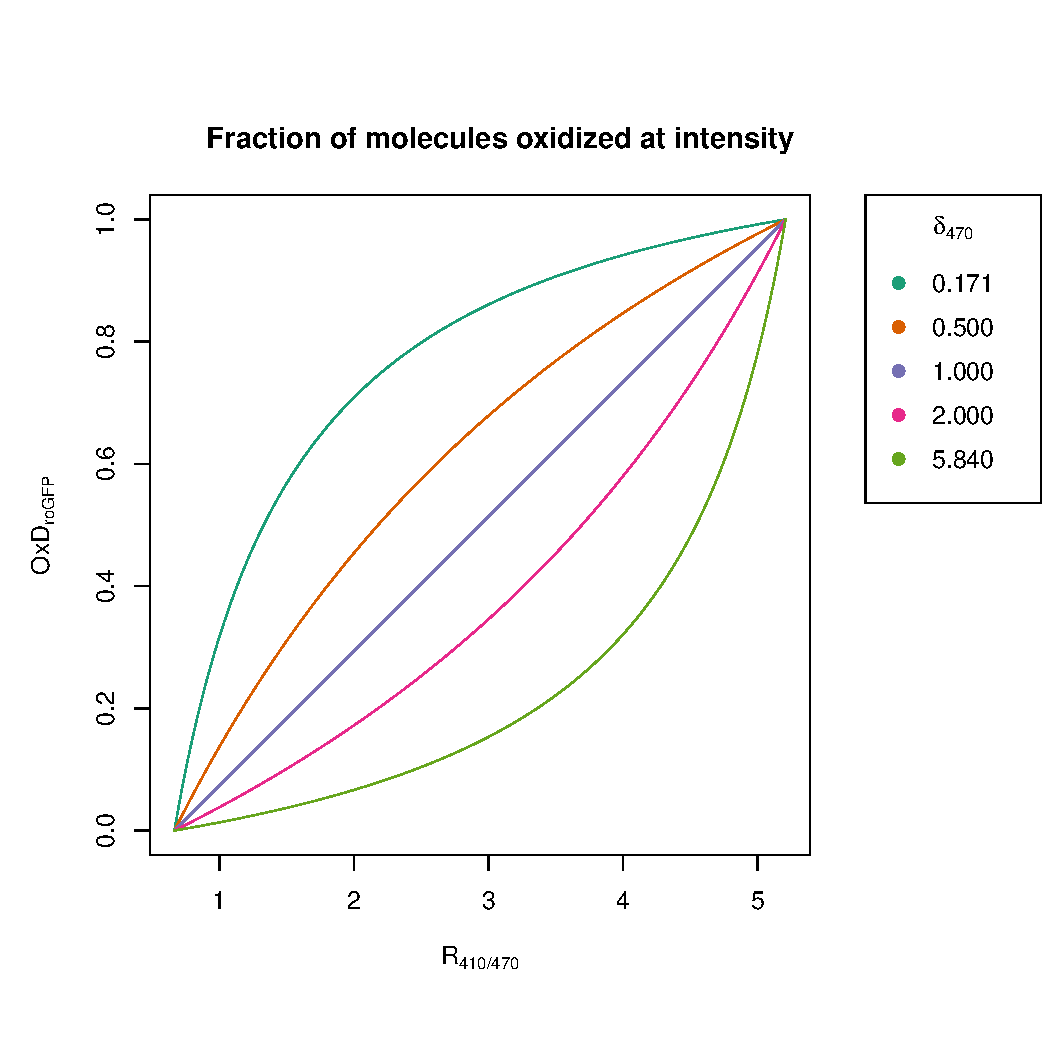
\includegraphics[page=1,width=.75\textwidth]{plot1.pdf}
    \caption{The relationship between observed intensity and OxD with different $\delta_{470}$ constants}
    \label{fig:my_label}
\end{figure}


\FloatBarrier

\section{Converting fraction of oxidized sensors into an electric potential}


\section{Reparameterizing the intensity ratio}


\end{document}


